\documentclass[12pt]{article}

% Paquetes necesarios
\usepackage[table]{xcolor} % Para colorear filas/columnas en tablas
\usepackage{graphicx}      % Para incluir imágenes
\usepackage{amsmath}       % Para ecuaciones matemáticas
\usepackage[a4paper, margin=1in]{geometry} % Configuración de página
\usepackage{tabularx}      % Para tablas con ajuste automático de ancho de columna
\usepackage{float}         % Para usar la opción [H] en tablas

\begin{document}

\begin{titlepage}
    \centering
    {\LARGE UNIVERSIDAD NACIONAL DE CÓRDOBA \par}
    \vspace{1cm}
    {\Large Facultad de Ciencias Exactas, Físicas y Naturales \par}
    \vspace{1.5cm}
    
\includegraphics[width=0.3\textwidth]{Logo-UNC.jpg} \par
    \vspace{1.5cm}
    {\LARGE \textbf{Trabajo Práctico Final - "Red de Petri / Agencia de Viajes"} \par}
    \vspace{1cm}
    {\Large \textbf{Programación Concurrente} \par}
    \vfill
    \textbf{Grupo:} \textit{Threading Bad} \par
    \vspace{0.5cm}
    - RODRIGUEZ, MATEO (43.967.398) \par
    - TRACHTA, AGUSTIN (43.271.890) \par
    \vfill
\end{titlepage}

\section{Introducción}
El presente informe detalla el trabajo realizado para abordar un problema de programación concurrente mediante el uso de redes de Petri y monitores. La programación concurrente se ha convertido en una disciplina esencial en el desarrollo de sistemas modernos, ya que permite aprovechar la capacidad de procesamiento de múltiples hilos de ejecución para mejorar la eficiencia y el rendimiento de las aplicaciones.

Sin embargo, la programación concurrente también presenta complejidades y desafíos únicos, como condiciones de carrera, bloqueos y problemas de sincronización. En este contexto, las redes de Petri emergen como una poderosa herramienta para modelar y analizar sistemas concurrentes, brindando una representación gráfica y formal de los estados y transiciones del sistema.

El objetivo principal de este informe es presentar el enfoque adoptado para resolver un problema específico de programación concurrente utilizando redes de Petri para modelar el sistema y monitores para gestionar la sincronización y el acceso seguro a los recursos compartidos. A lo largo del informe se hacen referencia a algunas definiciones que pasaremos a detallar ahora:

\section{¿Qué es una Red de Petri?}
Una Red de Petri (RdP) es un modelo matemático y gráfico utilizado para describir y analizar sistemas concurrentes y distribuidos.

\section{¿Por qué utilizamos RdP?}
Permiten modelar y visualizar casos de la vida real con paralelismo, concurrencia, sincronización e intercambio de recursos. Además, tienen un formalismo matemático y gráfico que nos permite determinar el disparo de una RdP y el siguiente marcado. Las RdP nos permiten separar la lógica de la política. La lógica es lo que puedo hacer, y la política es lo que me conviene hacer.

\section{Propiedades de la Red}
A continuación, se presentan las propiedades analizadas en la red de Petri, validadas mediante la herramienta \texttt{PIPE}. La figura inferior ilustra la red modelada:

\begin{center}
    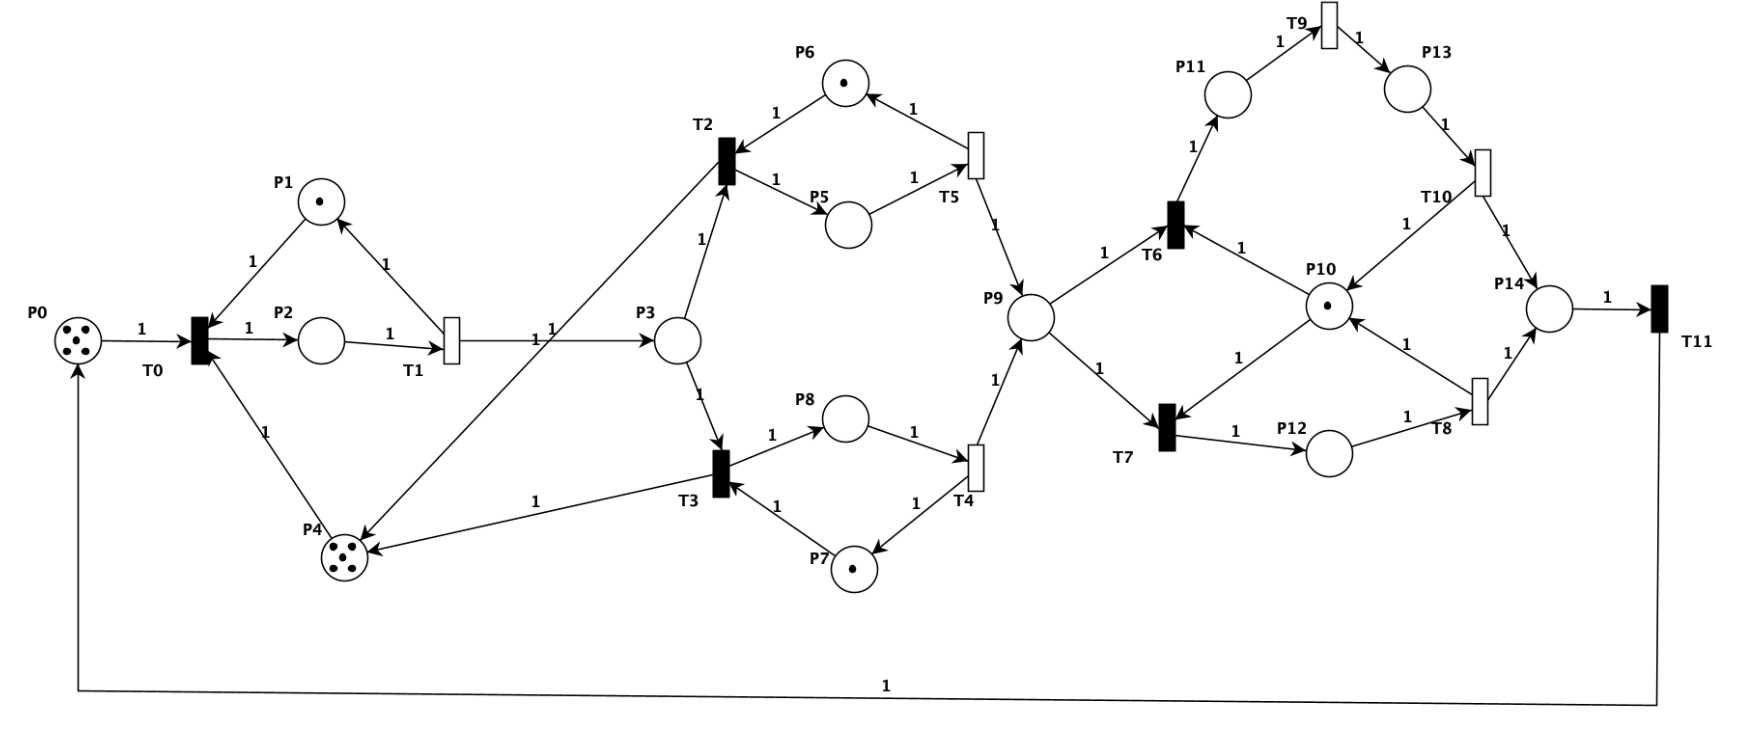
\includegraphics[width=0.9\textwidth]{Petri-Net.png}\\[0.5em]
    \textit{Figura: Red de Petri modelada.}
\end{center}

\bigskip

Adicionalmente, se muestran los resultados del análisis del espacio de estados de la red:

\begin{center}
    \textbf{Petri Net State Space Analysis Results}\\[0.5em]
    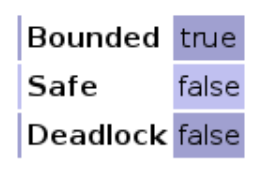
\includegraphics[width=0.4\textwidth]{Petri-Net-State.png}
\end{center}

\subsection{Red Limitada}
Una red de Petri es \textbf{limitada} si existe un límite superior para el número de tokens que pueden acumularse en cada plaza en cualquier marcado. Esto es fundamental para garantizar que los recursos representados por los tokens no se desborden.  
En este caso, la limitación se traduce en que la cantidad de clientes que pueden ingresar y ser atendidos está restringida por la capacidad del sistema (espacio físico, recursos humanos, etc.).

\subsection{Red Segura}
La red se considera \textbf{segura} si, en cualquier marcado alcanzable, cada plaza contiene como máximo un token.  
En nuestro modelo, se observa que algunas marcas pueden contener hasta 5 tokens, lo que indica que la red no es segura. Esto es coherente con el hecho de que se permite la entrada de hasta 5 clientes, lo que puede ser aceptable según la lógica del sistema, pero implica que la seguridad en el sentido estricto (máximo 1 token por plaza) no se cumple.

\subsection{Sin Deadlock y Vivacidad}
Un \textbf{deadlock} ocurre cuando la red alcanza un estado en el que ninguna transición es habilitada, lo que impide cualquier avance en la ejecución del sistema.  
El análisis realizado indica que la red no presenta deadlock, ya que en cada estado alcanzable existe al menos una transición habilitada. Esto garantiza que, sin importar el camino de ejecución, el sistema siempre puede continuar avanzando.  
Este comportamiento se relaciona con la \textbf{vivacidad} de la red: se asegura que, para cada transición, exista una secuencia de disparos que permita su eventual ejecución. En nuestro modelo, la vivacidad se corrobora al verificar que siempre hay transiciones disponibles para disparar, evitando estados bloqueados.

\bigskip

La validación de estas propiedades mediante \texttt{PIPE} nos proporciona confianza en el correcto comportamiento concurrente del sistema, asegurando que, a pesar de permitir múltiples tokens en algunas plazas, se mantienen las restricciones necesarias para evitar inconsistencias y bloqueos.

\section{Invariante de Transición}
Es un vector conformado por números enteros asociados a una secuencia de disparos. Son útiles para determinar propiedades estructurales de una RdP en forma analítica. Un invariante de transición es el conjunto mínimo de transiciones que, cuando las dispare, vuelvo al estado inicial. Esto nos indica que algo se hizo. Si me fijo cuántos invariantes se completaron, voy a entender cuántos ciclos se completaron.

\begin{center}
    \textbf{Petri net invariant analysis results}\\
    \textbf{T-Invariants}\\
    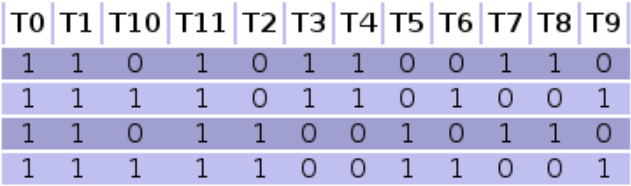
\includegraphics[width=0.8\textwidth]{T-invariants.png}\\
    \textit{The net is covered by positive T-invariants, therefore it might be bounded and live}
\end{center}

\section{Invariante de Plaza}
Un invariante de plaza es el conjunto de plazas en donde la suma de sus tokens se mantiene constante a lo largo de todos los marcados de la red.

\begin{center}
    \textbf{P-Invariants}\\
    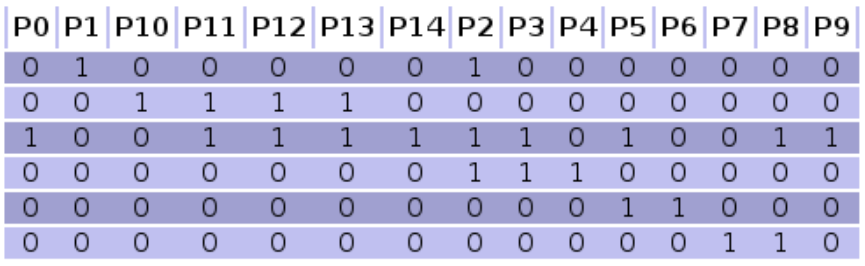
\includegraphics[width=0.8\textwidth]{P-invariants.png}\\
    \textit{The net is covered by positive T-invariants, therefore it is bounded.}
\end{center}

\subsection{Bounded and live}
El programa quiere decir que, además de estar acotada (bounded), la red siempre tiene la posibilidad de disparar alguna transición (live), por lo que no entra en un estado de bloqueo definitivo.

\subsection{Ecuaciones de Invariante de Plaza}
A continuación, se listan las ecuaciones de invariante de plaza derivadas de la red:

\[
M[P1] + M[P2] = 1
\]
\[
M[P10] + M[P11] + M[P12] + M[P13] = 1
\]
\[
M[P0] + M[P11] + M[P12] + M[P13] + M[P14] + M[P21] + M[P3] + M[P5] + M[P8] + M[P9] = 5
\]
\[
M[P2] + M[P3] + M[P4] = 5
\]
\[
M[P5] + M[P6] = 1
\]
\[
M[P7] + M[P8] = 1
\]

%---------------------------------
% NUEVA SECCIÓN: Tabla de estados
%---------------------------------
\section{Tabla de Estados en la Red de Petri}
En la siguiente tabla se detallan las plazas de la red de Petri y el estado que representan:

\begin{table}[H]
    \centering
    % Aumenta el espacio entre filas
    \renewcommand{\arraystretch}{1.2}
    \begin{tabularx}{\textwidth}{|c|X|}
    \hline
    \rowcolor{gray!20}
    \textbf{Plaza} & \textbf{Estado} \\ \hline
    P0  & Buffer de entrada de Clientes               \\ \hline
    P1  & Recursos compartidos del sistema            \\ \hline
    P2  & Cliente listo para entrar                   \\ \hline
    P3  & Cliente esperando a ser atendido            \\ \hline
    P4  & Recursos compartidos del sistema            \\ \hline
    P5  & Gestión de las Reservas                     \\ \hline
    P6  & Recursos compartidos del sistema            \\ \hline
    P7  & Gestión de las Reservas                     \\ \hline
    P8  & Recursos compartidos del sistema            \\ \hline
    P9  & Agente por cancelar la reserva              \\ \hline
    P10 & Agente por generar reserva                  \\ \hline
    P11 & Agente por confirmar reserva                \\ \hline
    P12 & Agente por pagar la reserva                 \\ \hline
    P13 & El cliente está por retirarse               \\ \hline
    P14 & (Lugar adicional según el modelo)           \\ \hline
    \end{tabularx}
    \caption{Tabla de estados en la red de Petri.}
    \label{tabla:estados-red-petri}
\end{table}

%---------------------------------
% NUEVA SECCIÓN: Tabla de eventos
%---------------------------------
\section{Tabla de Eventos en la Red de Petri}
A continuación se listan las transiciones y el evento asociado en la red de Petri:

\begin{table}[H]
    \centering
    \renewcommand{\arraystretch}{1.2}
    \begin{tabularx}{\textwidth}{|c|X|}
    \hline
    \rowcolor{green!20}
    \textbf{Transiciones} & \textbf{Evento} \\ \hline
    T0  & Input de Clientes                \\ \hline
    T1  & Cliente entra al negocio         \\ \hline
    T2  & Cliente es atendido              \\ \hline
    T3  & Cliente es atendido              \\ \hline
    T4  & Cliente pasa a la Confirmación   \\ \hline
    T5  & Cliente pasa a la Confirmación   \\ \hline
    T6  & Agente confirma la reserva       \\ \hline
    T7  & Agente rechaza la reserva        \\ \hline
    T8  & Cliente pasa a retirarse         \\ \hline
    T9  & Se paga la reserva               \\ \hline
    T10 & Cliente pasa a retirarse         \\ \hline
    T11 & Cliente se retira de la agencia  \\ \hline
    \end{tabularx}
    \caption{Tabla de eventos en la red de Petri.}
    \label{tabla:eventos-red-petri}
\end{table}


\section{Determinación de la cantidad de hilos}

Para determinar la cantidad máxima de hilos activos simultáneamente en el sistema, se aplicó el algoritmo propuesto por el profesor, el cual se basa en el análisis de los invariantes de transición (IT) de la red de Petri. Este método permite descomponer la ejecución en trayectorias independientes, facilitando la asignación de hilos según la concurrencia en cada segmento. A continuación, se detalla el procedimiento seguido:

\subsection{Obtención de los Invariantes de Transición (IT)}
Se han identificado los siguientes IT de la tabla mencionada en el apartado 5:
\begin{enumerate}
    \item $\{T0, T1, T3, T4, T7, T8, T11\}$
    \item $\{T0, T1, T3, T4, T6, T9, T10, T11\}$
    \item $\{T0, T1, T2, T5, T7, T8, T11\}$
    \item $\{T0, T1, T2, T5, T6, T9, T10, T11\}$
\end{enumerate}

\subsection{Obtención del Conjunto de Plazas Asociadas a cada IT}
Para cada IT, se identifica el conjunto de plazas involucradas, lo que permite analizar cómo se distribuyen los recursos y estados en el sistema. 
\begin{enumerate}
    \item Para el IT1: $\{P0, P1, P2, P3, P4, P7, P8, P9, P10, P12, P14\}$
    \item Para el IT2: $\{P0, P1, P2, P3, P4, P7, P8, P9, P10, P11, P13, P14\}$
    \item Para el IT3: $\{P0, P1, P2, P3, P4, P5, P6, P9, P10, P12, P14\}$
    \item Para el IT4: $\{P0, P1, P2, P3, P4, P5, P6, P9, P10, P11, P13, P14\}$
\end{enumerate}

\subsection{Determinación de las Plazas de Acción}
Dentro de cada IT, se elimina el conjunto de plazas que representan restricciones, recursos o estados idle, dejando únicamente aquellas plazas asociadas a acciones críticas. Así se obtienen:
\begin{enumerate}
    \item Para el IT1: $\{P2, P8, P12\}$
    \item Para el IT2: $\{P2, P8, P11, P13\}$
    \item Para el IT3: $\{P2, P5, P12\}$
    \item Para el IT4: $\{P2, P5, P11, P13\}$
\end{enumerate}

\subsection{Construcción del Conjunto de Estados del Conjunto de Plazas de Acción (PA)}
Se define el conjunto PA como la unión de todas las plazas de acción obtenidas:
\[
PA = \{P2, P5, P8, P11, P12, P13\}
\]
A partir del árbol de alcanzabilidad de la red de Petri, se extraen todos los marcados (estados) posibles correspondientes a este conjunto.

\subsection{Cálculo del Valor Máximo de Hilos Simultáneos}
Para cada marcado en el conjunto PA se calcula la suma total de tokens. El valor máximo obtenido en estas sumas representa la cantidad máxima de hilos que pueden estar activos simultáneamente en el sistema. En nuestro caso, se determinó que:
\[
\textbf{Valor máximo de hilos simultáneos} = 4
\]

Este resultado indica que, en el punto de mayor concurrencia, hasta 4 hilos pueden ejecutarse de forma simultánea, lo que permite aprovechar de manera óptima los recursos disponibles.

\vspace{1em}
\textbf{Referencia:} Los algoritmos y el procedimiento descrito se basan en el informe proporcionado por el profesor (ver Referencias al final del informe).


\section{Red de Petri final}

La red de Petri final utilizada en el programa consta de 6 segmentos.
\begin{center}
    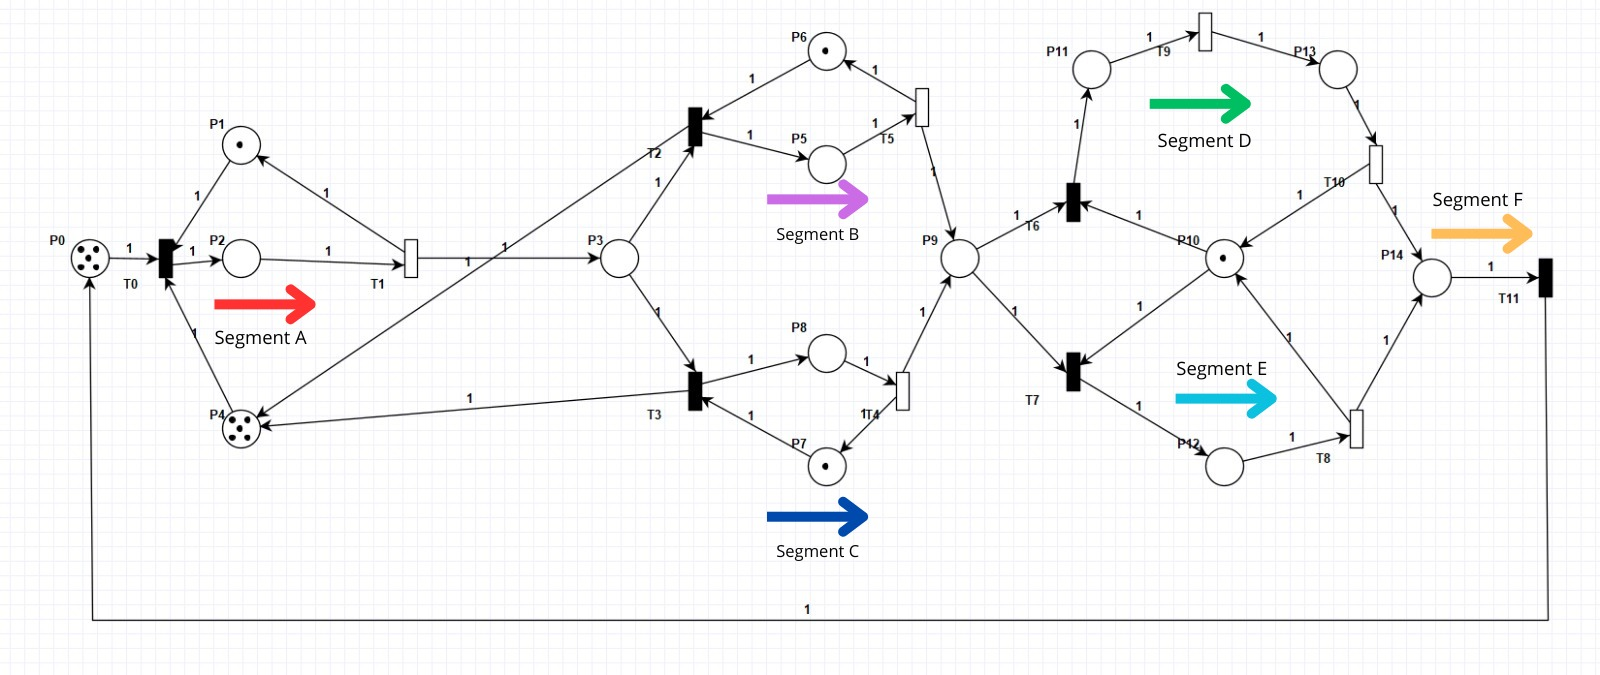
\includegraphics[width=0.9\textwidth]{Petri-Net-Final.jpeg}
\end{center}

\section{Justificación de la elección de los segmentos}

La elección de los segmentos en la red de Petri se basó en la identificación de estructuras lineales, forks y joins en la red. Cada segmento se definió con el objetivo de maximizar la concurrencia y optimizar el uso de los hilos disponibles:

\begin{enumerate}
    \item \textbf{Segmento A:} Es una secuencia de transiciones sin bifurcaciones, por lo que se ejecuta de manera secuencial sin interferencias.
    
    \item \textbf{Segmentos B, C, D, E:} Estos segmentos contienen transiciones que generan caminos en paralelo (forks). Al dividir la ejecución en hilos independientes, se evita que un solo hilo tenga que decidir qué camino seguir, delegando la decisión a la política de ejecución del sistema.
    
    \item \textbf{Segmento D:} Aunque es parte de un fork, en su parte final no comparte transiciones con otros segmentos, por lo que actúa también como un segmento lineal.
    
    \item \textbf{Segmento F:} Representa el punto de convergencia de caminos en la red (join). Para evitar bloqueos, se permite la ejecución paralela de los segmentos anteriores, asegurando que todas las dependencias se resuelvan antes de continuar con la ejecución final.
\end{enumerate}

\section{Determinación de hilos máximos por segmento}

A partir de la segmentación de la red de Petri y la identificación de los subconjuntos de plazas asociadas a cada segmento, se determina la cantidad máxima de hilos que pueden ejecutarse simultáneamente. La segmentación permite dividir la ejecución en partes independientes, asegurando que no haya interferencias en la ejecución concurrente.

Cada segmento tiene un conjunto de plazas asociadas, denominadas \(PS_i\), que representan los estados alcanzables en dicho segmento. A continuación, se presentan los segmentos con sus respectivas plazas y la cantidad máxima de hilos necesarios para su ejecución:

\begin{itemize}
    \item \(PS_a = \{P2\} \Rightarrow \text{MAX} = 1\)
    \item \(PS_b = \{P5\} \Rightarrow \text{MAX} = 1\)
    \item \(PS_c = \{P8\} \Rightarrow \text{MAX} = 1\)
    \item \(PS_d = \{P11, P13\} \Rightarrow \text{MAX} = 1\)
    \item \(PS_e = \{P12\} \Rightarrow \text{MAX} = 1\)
    \item \(PS_f = \{P14\} \Rightarrow \text{MAX} = 1\)
\end{itemize}

Dado que cada segmento requiere un hilo para su ejecución, la suma de los hilos necesarios en todos los segmentos nos da la cantidad total de hilos que el sistema puede necesitar en toda su ejecución:

\[
Hilos\ totales\ del\ sistema = 1 + 1 + 1 + 1 + 1 + 1 = 6
\]

Sin embargo, esto no significa que en todo momento haya 6 hilos ejecutándose en simultáneo.  
El primer algoritmo determinó que la **máxima cantidad de hilos activos simultáneamente** en la red de Petri es **4**, lo que significa que en el punto de mayor concurrencia del sistema, pueden llegar a ejecutarse hasta 4 hilos a la vez.  
La segmentación realizada permite distribuir la carga de trabajo de manera eficiente, asegurando que cada hilo ejecute su parte sin interferencias y maximizando el rendimiento del sistema.

\section{Implementación en Java}

En esta sección se describe la implementación en Java del sistema, haciendo especial énfasis en cómo se tradujo el modelo teórico de la red de Petri a una solución práctica y concurrente. El sistema se organiza en varios paquetes, entre los que se destacan: \texttt{monitor}, \texttt{petrinet}, \texttt{utils} y \texttt{pool}. A continuación, se detalla el funcionamiento del paquete \texttt{petrinet}, que constituye el núcleo del modelo.

\subsection{Paquete \texttt{petrinet}}

El paquete \texttt{petrinet} es el núcleo de la simulación de la red de Petri y se encarga de modelar su comportamiento teórico en un entorno concurrente. En este paquete se definen las clases principales que gestionan el estado de la red, las reglas de disparo (transiciones) y la ejecución de segmentos de la red. A continuación se describen sus componentes:

\subsubsection{Clase \texttt{Places}}

La clase \texttt{Places} representa el conjunto de plazas de la red de Petri y gestiona el conteo de tokens en cada una de ellas. Sus responsabilidades principales son:
\begin{itemize}
    \item \textbf{Manejo del estado:} Mantener un mapa (\texttt{HashMap}) que asocia cada identificador de plaza con la cantidad de tokens presentes.
    \item \textbf{Sincronización:} Utiliza un bloqueo global (proporcionado por \texttt{TransitionNotifier.lock}) para asegurar la exclusión mutua en las operaciones de lectura y escritura, evitando condiciones de carrera.
    \item \textbf{Operaciones básicas:} 
    \begin{itemize}
        \item \texttt{addPlace(int placeId, int initialTokens)}: Agrega una plaza con un número inicial de tokens.
        \item \texttt{getTokenCount(int placeId)}: Devuelve la cantidad de tokens en una plaza, protegiendo la operación mediante bloqueo.
        \item \texttt{addTokens(int placeId, int count)} y \texttt{removeTokens(int placeId, int count)}: Modifican la cantidad de tokens y notifican a los hilos en espera mediante la condición \texttt{transitionsEnabled}.
        \item \texttt{checkInvariants()}: Recorre todas las plazas para verificar que no existan violaciones (por ejemplo, que no haya valores negativos), manteniendo la integridad del modelo.
    \end{itemize}
\end{itemize}

\subsubsection{Clase \texttt{Transition}}

La clase \texttt{Transition} encapsula la definición de una transición en la red de Petri, es decir, una regla que define cómo se modifican los tokens al dispararse:
\begin{itemize}
    \item \textbf{Precondiciones y Postcondiciones:} Se modelan como mapas que asocian el identificador de cada plaza con la cantidad de tokens requeridos (precondiciones) o a añadir (postcondiciones).
    \item \textbf{Transiciones Temporales:} Permite definir transiciones con retardo. Si una transición es temporal, se introduce un retraso (delay) en milisegundos antes de aplicar las modificaciones en el estado.
    \item \textbf{Verificación de habilitación:} El método \texttt{isEnabled(Places places)} comprueba que en cada plaza se cumplen las precondiciones (tokens suficientes) para permitir el disparo.
    \item \textbf{Disparo de la transición:} El método \texttt{fire(Places places)} valida la habilitación, espera el retardo en caso de ser temporal, y procede a remover tokens de las plazas de entrada y añadir tokens en las plazas de salida, modificando así el estado de la red.
\end{itemize}

\subsubsection{Clase \texttt{Segment}}

La clase \texttt{Segment} representa un segmento de ejecución de la red de Petri, es decir, un conjunto de transiciones agrupadas que se ejecutan como una unidad:
\begin{itemize}
    \item \textbf{Agrupación de Transiciones:} Cada segmento contiene una lista de transiciones que, según la lógica del modelo, deben dispararse en conjunto.
    \item \textbf{Implementación de \texttt{Runnable}:} Permite que cada segmento sea gestionado por un planificador central (a través del monitor), ejecutándose en hilos independientes.
    \item \textbf{Sincronización interna:} Se utiliza un flag \texttt{isRunning} para evitar que el mismo segmento se ejecute de forma concurrente en más de un hilo.
    \item \textbf{Comprobación de habilitación:} El método \texttt{hasEnabledAndAllowedTransition()} verifica, consultando la política definida en el monitor, que al menos una transición del segmento está habilitada y permitida.
    \item \textbf{Ejecución:} En el método \texttt{run()}, el segmento itera sobre sus transiciones y, para cada una habilitada, solicita al monitor que dispare la transición mediante el método \texttt{fireTransition}.
\end{itemize}

\subsubsection{Interacción y Sincronización Global}

El diseño del paquete \texttt{petrinet} se integra de forma coordinada con otros componentes del sistema:
\begin{itemize}
    \item La clase \texttt{Places} actúa como repositorio global del estado de la red, sobre el cual operan las transiciones.
    \item La clase \texttt{Transition} utiliza \texttt{Places} para leer y modificar el estado, respetando las condiciones de sincronización mediante bloqueos.
    \item Los segmentos, representados por la clase \texttt{Segment}, agrupan transiciones y se gestionan a través del monitor, que decide la ejecución basada en la política de resolución de conflictos.
    \item Se utiliza un \texttt{Logger} para trazar eventos y facilitar la depuración, lo que ayuda a verificar el correcto funcionamiento y a identificar posibles errores.
\end{itemize}

\subsection{Paquete \texttt{monitor}}

El paquete \texttt{monitor} se encarga de coordinar la ejecución de las transiciones de la red de Petri, implementando un mecanismo central de sincronización y resolución de conflictos. Para ello, se define la clase \texttt{Monitor} que expone el método único \texttt{fireTransition}, y se utiliza un Scheduler para la gestión de segmentos de la red. Asimismo, se implementan diferentes políticas (\texttt{BalancedPolicy} y \texttt{PriorityPolicy}) para resolver conflictos y asignar prioridades en la ejecución de transiciones. A continuación, se describen los componentes principales de este paquete.

\subsubsection{Clase \texttt{Scheduler}}

La clase \texttt{Scheduler} es un hilo dedicado que supervisa continuamente los segmentos definidos en la red de Petri y los envía al administrador de hilos (\texttt{PoolManager}) cuando detecta que alguno de ellos tiene transiciones habilitadas para disparar. Sus características principales son:
\begin{itemize}
    \item \textbf{Monitoreo de segmentos:} Recorre la lista de segmentos y verifica, mediante el método \texttt{canBeScheduled()}, si alguno de ellos tiene al menos una transición habilitada.
    \item \textbf{Sincronización eficiente:} Utiliza un \texttt{ReentrantLock} y una condición (\texttt{transitionsEnabled}) definida en la clase \texttt{TransitionNotifier} para esperar que haya algun movimiento de tokens en las plazas del sistema cuando no hay segmentos listos, evitando ciclos de espera activa.
    \item \textbf{Terminación controlada:} Proporciona un método \texttt{stop()} que permite finalizar la ejecución del Scheduler de forma segura, notificando a cualquier hilo que se encuentre en espera.
\end{itemize}

El método \texttt{run()} del Scheduler itera sobre los segmentos y, si ninguno está listo, se bloquea esperando una señal. Esta señal se envía desde otros componentes cuando el estado de las transiciones cambia (al agregar  en las plazas).

\subsubsection{Clase \texttt{Monitor}}

La clase \texttt{Monitor} actúa como el coordinador central del sistema y se encarga de:
\begin{itemize}
    \item \textbf{Fijar la sincronización:} El método \texttt{fireTransition} es el único método público y se utiliza para disparar transiciones. Este método es sincronizado para asegurar un acceso seguro y exclusivo al estado compartido.
    \item \textbf{Consulta de habilitación y políticas:} Antes de disparar una transición, el Monitor consulta si la transición está habilitada (mediante el método \texttt{isEnabled} de la clase \texttt{Transition}) y, además, verifica que la política activa permita su ejecución.
    \item \textbf{Actualización de contadores:} Tras el disparo exitoso de una transición, se actualizan los contadores internos mediante el método \texttt{updateCounters} de la política, lo que permite llevar un registro del balance o la prioridad en la ejecución.
    \item \textbf{Gestión del Scheduler:} El Monitor es responsable de iniciar y detener el Scheduler, integrándolo con el administrador de hilos (\texttt{PoolManager}) para garantizar que los segmentos se ejecuten en función de la disponibilidad de transiciones.
\end{itemize}

Dentro del método \texttt{fireTransition}, se realiza el siguiente flujo:
\begin{enumerate}
    \item Se recupera la transición asociada al identificador.
    \item Se vuelve a verificar que la transición esté habilitada en función de los tokens presentes en las \texttt{Places}.
    \item Se consulta nuevamente la política para confirmar que el disparo es permitido.
    \item Se dispara la transición, aplicando las precondiciones y postcondiciones sobre las \texttt{Places}.
    \item Se actualizan los contadores de la política y se comprueban los invariantes del sistema.
    \item Se suma un contador sobre la transicion 0 de tal forma que al llegar a 187 (es decir, 186 cilos, o invariantes de transicion completados) todos los hilos son notificados y se termina el sistema.
\end{enumerate}

\subsubsection{Interfaces y Políticas}

El Monitor utiliza interfaces para definir la estructura de la política y la forma de coordinar el disparo de transiciones:
\begin{itemize}
    \item \textbf{Interfaz \texttt{MonitorInterface}:} Define el método \texttt{fireTransition(int transition)} que es el punto de entrada para disparar transiciones.
    \item \textbf{Interfaz \texttt{Policy}:} Establece dos métodos: \texttt{allowTransition(int transitionId, Places places)} para decidir si una transición puede dispararse, y \texttt{updateCounters(int transitionId, Places places)} para actualizar el estado interno tras el disparo.
\end{itemize}

Se implementan dos políticas principales:
\begin{enumerate}
    \item \textbf{BalancedPolicy:}  
    \begin{itemize}
        \item \textbf{Objetivo:} Garantizar un equilibrio en la atención entre el agente de reservas superior (transición 2) y el inferior (transición 3). De igual forma, balancear el número de confirmaciones y cancelaciones.
        \item \textbf{Implementación:} Se utilizan contadores internos para cada tipo de operación. Por ejemplo, la política permite disparar la transición asociada al agente superior solo si su contador es menor o igual al del agente inferior.
    \end{itemize}
    \item \textbf{PriorityPolicy:}  
    \begin{itemize}
        \item \textbf{Objetivo:} Priorizar el procesamiento del agente superior y la confirmación de reservas. Se requiere que el agente superior genere al menos el 75\% de las reservas y que las confirmaciones representen al menos el 80\% del total.
        \item \textbf{Implementación:} Se calculan ratios basados en los contadores internos y se permite o bloquea el disparo de ciertas transiciones en función de estos porcentajes.
    \end{itemize}
\end{enumerate}

Ambas políticas se integran en el Monitor, de modo que al disparar una transición se consulta la política activa. Esto garantiza que la lógica de resolución de conflictos y asignación de prioridades se mantiene separada de la lógica de disparo y la actualización del estado, facilitando la modularidad y el mantenimiento del código.

\subsubsection{Interacción Global en el Paquete \texttt{monitor}}

La interacción entre el Scheduler, el Monitor y las políticas es fundamental para el correcto funcionamiento del sistema:
\begin{itemize}
    \item El \texttt{Scheduler} monitorea continuamente los segmentos de la red y, cuando alguno tiene transiciones habilitadas, los envía al administrador de hilos para su ejecución.
    \item El \texttt{Monitor}, mediante el método \texttt{fireTransition}, se encarga de coordinar el disparo de las transiciones, integrando la consulta a la política y la actualización del estado.
    \item Las políticas (\texttt{BalancedPolicy} y \texttt{PriorityPolicy}) permiten gestionar de forma dinámica los conflictos y asegurar que se cumplan los criterios de balance y prioridad definidos, actualizando internamente los contadores que determinan si se permite el disparo de una transición.
\end{itemize}

En conjunto, el paquete \texttt{monitor} garantiza que la ejecución de la red de Petri se realice de forma ordenada, segura y eficiente, permitiendo la resolución de conflictos y la maximización del paralelismo a través de la coordinación de hilos y la aplicación de políticas específicas.

\subsection{Paquete \texttt{pool}}

El paquete \texttt{pool} se encarga de la gestión y administración del pool de hilos, permitiendo la ejecución concurrente de tareas. Este paquete implementa dos componentes principales: un \texttt{ThreadFactory} personalizado y un administrador del pool de hilos (\texttt{PoolManager}).

\subsubsection{Clase \texttt{MyThreadFactory}}

La clase \texttt{MyThreadFactory} implementa la interfaz \texttt{ThreadFactory} y se utiliza para crear hilos con un nombre específico, facilitando la identificación y depuración de los mismos. Sus características principales son:
\begin{itemize}
    \item \textbf{Nombre base para hilos:} Permite asignar un nombre base a los hilos creados, seguido de un contador incremental, lo que genera nombres únicos (por ejemplo, \texttt{"ThreadPool-1"}, \texttt{"ThreadPool-2"}, etc.).
    \item \textbf{Atomicidad:} Utiliza un objeto \texttt{AtomicInteger} para asegurar que el contador de hilos se incremente de forma segura en entornos concurrentes.
    \item \textbf{Personalización:} Se pueden configurar propiedades adicionales de los hilos (como el estado daemon) en el método \texttt{newThread}, adaptándose a las necesidades del sistema.
\end{itemize}

\subsubsection{Clase \texttt{PoolManager}}

La clase \texttt{PoolManager} encapsula la lógica para la administración del pool de hilos, utilizando un \texttt{ExecutorService} con un número fijo de hilos. Sus responsabilidades incluyen:
\begin{itemize}
    \item \textbf{Inicialización del pool:} Configura un pool de hilos fijo mediante \texttt{Executors.newFixedThreadPool}, utilizando el \texttt{MyThreadFactory} para la creación de hilos.
    \item \textbf{Envío de tareas:} Proporciona el método \texttt{submitTask(Runnable task)} para enviar tareas al pool de hilos, permitiendo la ejecución concurrente de las mismas.
    \item \textbf{Cierre del pool:} Implementa métodos para la terminación controlada del pool (\texttt{shutdown()}), esperando a que las tareas en ejecución finalicen, o bien para un cierre inmediato (\texttt{shutdownNow()}), cancelando las tareas en curso.
\end{itemize}

En conjunto, el paquete \texttt{pool} proporciona una infraestructura robusta para la gestión de hilos, lo que es crucial para la ejecución concurrente del sistema. La integración de un \texttt{ThreadFactory} personalizado con el \texttt{PoolManager} asegura que las tareas se ejecuten de forma ordenada y se puedan rastrear fácilmente durante la ejecución, lo que resulta fundamental para la depuración y optimización de la aplicación.

\subsection{Paquete \texttt{utils}}

El paquete \texttt{utils} proporciona herramientas de apoyo fundamentales para el correcto funcionamiento del sistema. Entre ellas se incluyen un Logger para la depuración y registro de eventos, la construcción de la red de Petri a través de la clase \texttt{PetriNet}, y un mecanismo de notificación de cambios en la red, implementado en la clase \texttt{TransitionNotifier}.

\subsubsection{Clase \texttt{Logger}}

La clase \texttt{Logger} es una implementación sencilla y thread-safe de un registrador (logger). Se implementa como un singleton, lo que garantiza que exista un único punto de registro en la aplicación. Entre sus características se destacan:
\begin{itemize}
    \item \textbf{Formato de registro:} Cada entrada de log sigue el formato:
    \begin{center}
        \texttt{[YYYY-MM-DD HH:MM:SS] [Thread-Name] [LEVEL] Message}
    \end{center}
    \item \textbf{Métodos de registro:} Se proporcionan métodos para registrar mensajes de distintos niveles (INFO, DEBUG, WARN, ERROR). Cada método utiliza el mismo método privado \texttt{log} para formatear y escribir la entrada en el archivo \texttt{petri\_net.log}.
    \item \textbf{Sincronización:} Los métodos de registro son sincronizados para asegurar que múltiples hilos puedan escribir en el archivo de log sin interferencias.
\end{itemize}

\subsubsection{Clase \texttt{TransitionNotifier}}

La clase \texttt{TransitionNotifier} es esencial para la coordinación de la red de Petri. Esta clase centraliza dos elementos críticos para la sincronización:
\begin{itemize}
    \item \textbf{ReentrantLock:} Se utiliza para proteger las operaciones que modifican el estado de la red, evitando condiciones de carrera.
    \item \textbf{Condition \texttt{transitionsEnabled}:} Esta condición permite notificar a los hilos que están esperando cambios en el estado de la red (por ejemplo, cuando se agregan o quitan tokens en las \texttt{Places}). Cada vez que se actualiza el estado de la red, se llama a \texttt{signalAll()} para despertar a los hilos que esperan que alguna transición se habilite.
\end{itemize}
De esta forma, \texttt{TransitionNotifier} actúa como un mecanismo central de señalización, facilitando la coordinación entre el Monitor, el Scheduler y los segmentos que esperan poder disparar sus transiciones.

\subsubsection{Clase \texttt{PetriNet}}

La clase \texttt{PetriNet} encapsula el proceso de construcción de la red de Petri. Su función es:
\begin{itemize}
    \item \textbf{Inicializar el modelo:} Crea las instancias de \texttt{Places}, define las transiciones (con sus precondiciones, postcondiciones y, en algunos casos, retardo temporal) y agrupa estas transiciones en segmentos de ejecución.
    \item \textbf{Integrar componentes:} Establece la relación entre las \texttt{Places}, las \texttt{Transition}, los segmentos y el Monitor, asegurando que el modelo se construya de acuerdo a la especificación.
    \item \textbf{Selección de políticas:} Permite elegir entre distintas políticas de resolución de conflictos (por ejemplo, \texttt{BalancedPolicy} o \texttt{PriorityPolicy}) que se aplicarán en el Monitor.
\end{itemize}
\subsection{Clase \texttt{Main}}

La clase \texttt{Main} es el punto de entrada de la aplicación y coordina la ejecución de la simulación de la red de Petri. A continuación se describe el flujo principal implementado en el método \texttt{main}:

\begin{enumerate}
    \item \textbf{Inicialización y registro:}  
    Se obtiene la instancia del \texttt{Logger} (implementado como singleton) para comenzar a registrar los eventos de la ejecución, y se registra el inicio de la simulación.

    \item \textbf{Construcción de la red de Petri:}  
    Se crea una instancia de la clase \texttt{PetriNet} (del paquete \texttt{utils}), la cual se encarga de construir el modelo: inicializar las \texttt{Places}, definir las \texttt{Transitions} (incluyendo sus precondiciones, postcondiciones y retardo para transiciones temporales) y agruparlas en \texttt{Segments}. Además, se configura el \texttt{Monitor} y se selecciona la política a utilizar (en este ejemplo se opta por \texttt{PriorityPolicy}, aunque también se podría utilizar \texttt{BalancedPolicy}).

    \item \textbf{Configuración de la concurrencia:}  
    Se extraen los segmentos, las \texttt{Places} y el \texttt{Monitor} del objeto \texttt{PetriNet}. A continuación, se crea un \texttt{PoolManager} utilizando un \texttt{MyThreadFactory} personalizado que asigna nombres a los hilos, y se configura el pool con 4 hilos. Esta configuración permite ejecutar las tareas (segmentos) de forma concurrente.

    \item \textbf{Inicio del Scheduler:}  
    El \texttt{Monitor} inicia el Scheduler (del paquete \texttt{monitor}), el cual se encarga de enviar los segmentos al \texttt{PoolManager} cuando tienen transiciones habilitadas. De este modo, el sistema comienza a disparar transiciones según las reglas de la red y la política de resolución de conflictos.

    \item \textbf{Espera de la condición de invariante:}  
    La clase \texttt{Main} se bloquea esperando que se cumpla la condición invariante (en este caso, que la transición de inicio, T0, se dispare 187 veces). Para ello, se utiliza el lock proporcionado por el \texttt{Monitor} (mediante \texttt{getInvariantLock()}) y se espera a que se notifique el cumplimiento de dicha condición.

    \item \textbf{Finalización de la simulación:}  
    Una vez alcanzada la condición (186 invariantes completados), se detiene el Scheduler y se cierra inmediatamente el pool de hilos. Seguidamente, se mide y registra el tiempo total de ejecución.

    \item \textbf{Impresión de resultados:}  
    Se muestran en la salida estándar los tokens finales presentes en cada una de las \texttt{Places} y, dependiendo de la política utilizada, se imprimen los contadores asociados a las transiciones relevantes (por ejemplo, los contadores de reservas superiores, inferiores, confirmadas y canceladas). Además, se calculan y muestran algunos invariantes derivados de estos contadores.

    \item \textbf{Cierre del Logger:}  
    Finalmente, se registra el final de la simulación y se cierra el Logger, liberando los recursos asociados.
\end{enumerate}

La clase \texttt{Main} orquesta la puesta en marcha del sistema, integrando la construcción del modelo, la configuración de la concurrencia y la coordinación mediante el Monitor y el Scheduler, y finalmente, la recogida de resultados para su análisis. Esto demuestra la integración completa del modelo teórico de la red de Petri con la implementación práctica en Java, cumpliendo con los requerimientos del proyecto.

\section{Análisis de los Resultados}

Se realizaron diversas pruebas modificando los tiempos de demora en las transiciones para evaluar el impacto de las políticas \textbf{Balanced} y \textbf{Priority}. A continuación, se presentan los resultados obtenidos para cada configuración:

\subsection{Caso 1: Todas las transiciones con 5 ms}

\begin{figure}[H]
    \centering
    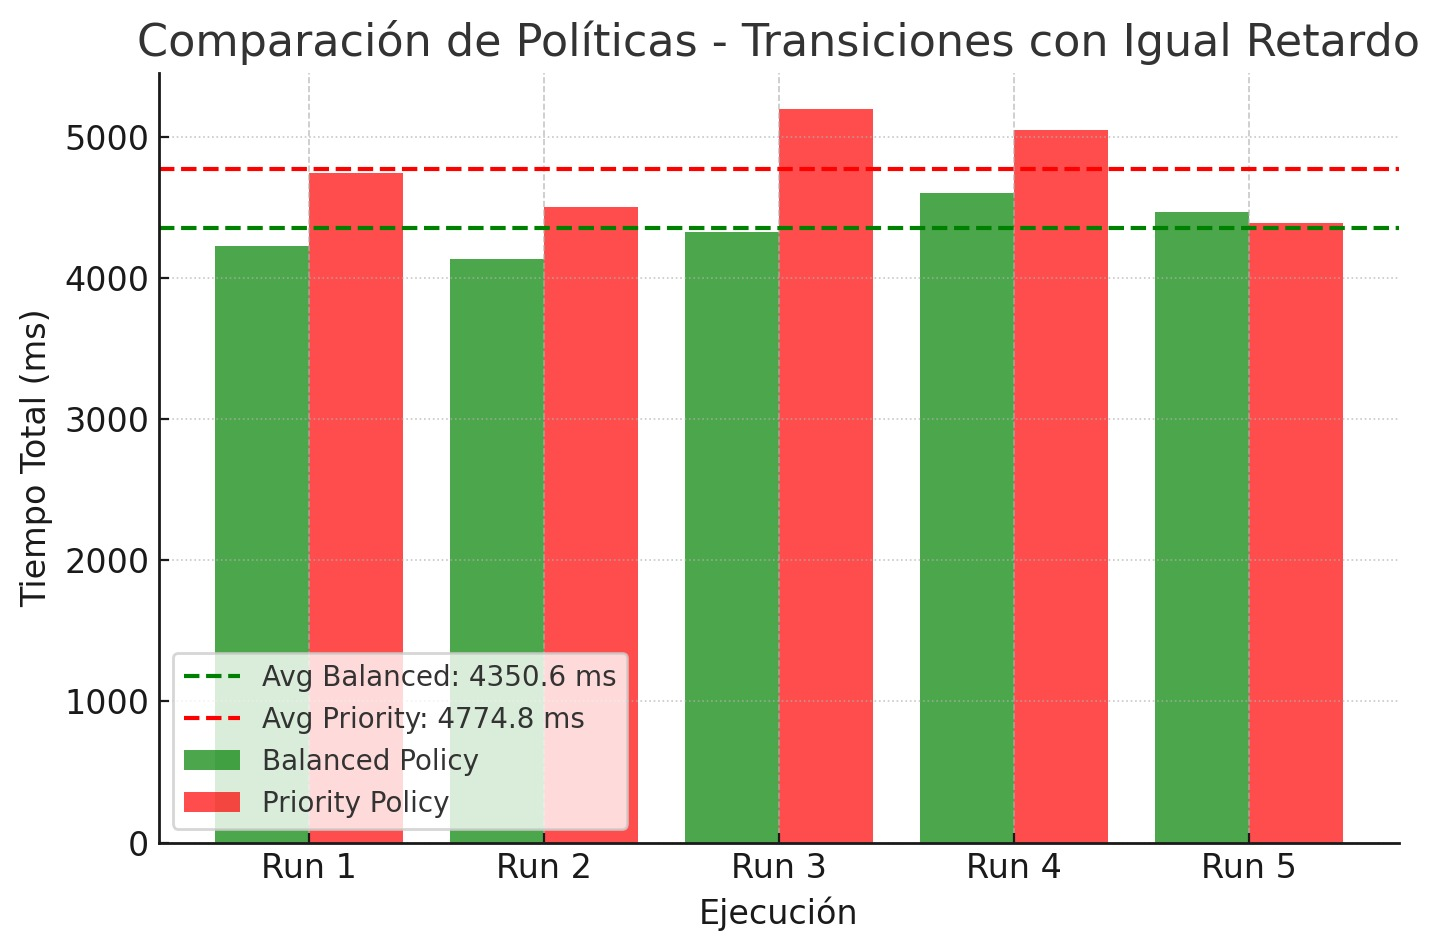
\includegraphics[width=0.7\textwidth]{CASO_1.jpeg}
    \caption{Resultados del Caso 1.}
\end{figure}

En este caso, todas las transiciones tienen el mismo tiempo de demora (\textbf{5 ms}), lo que significa que ninguna transición representa un cuello de botella significativo. Los tiempos de ejecución son similares, aunque la política \textbf{Balanced} muestra un tiempo menor (\textbf{4350.6 ms}) en comparación con \textbf{Priority} (\textbf{4774.8 ms}). Esto se debe a que \textbf{Priority} prioriza ciertos segmentos, lo que en este caso no aporta una ventaja significativa.

\subsection{Caso 2: Demora en el pago}

\begin{figure}[H]
    \centering
    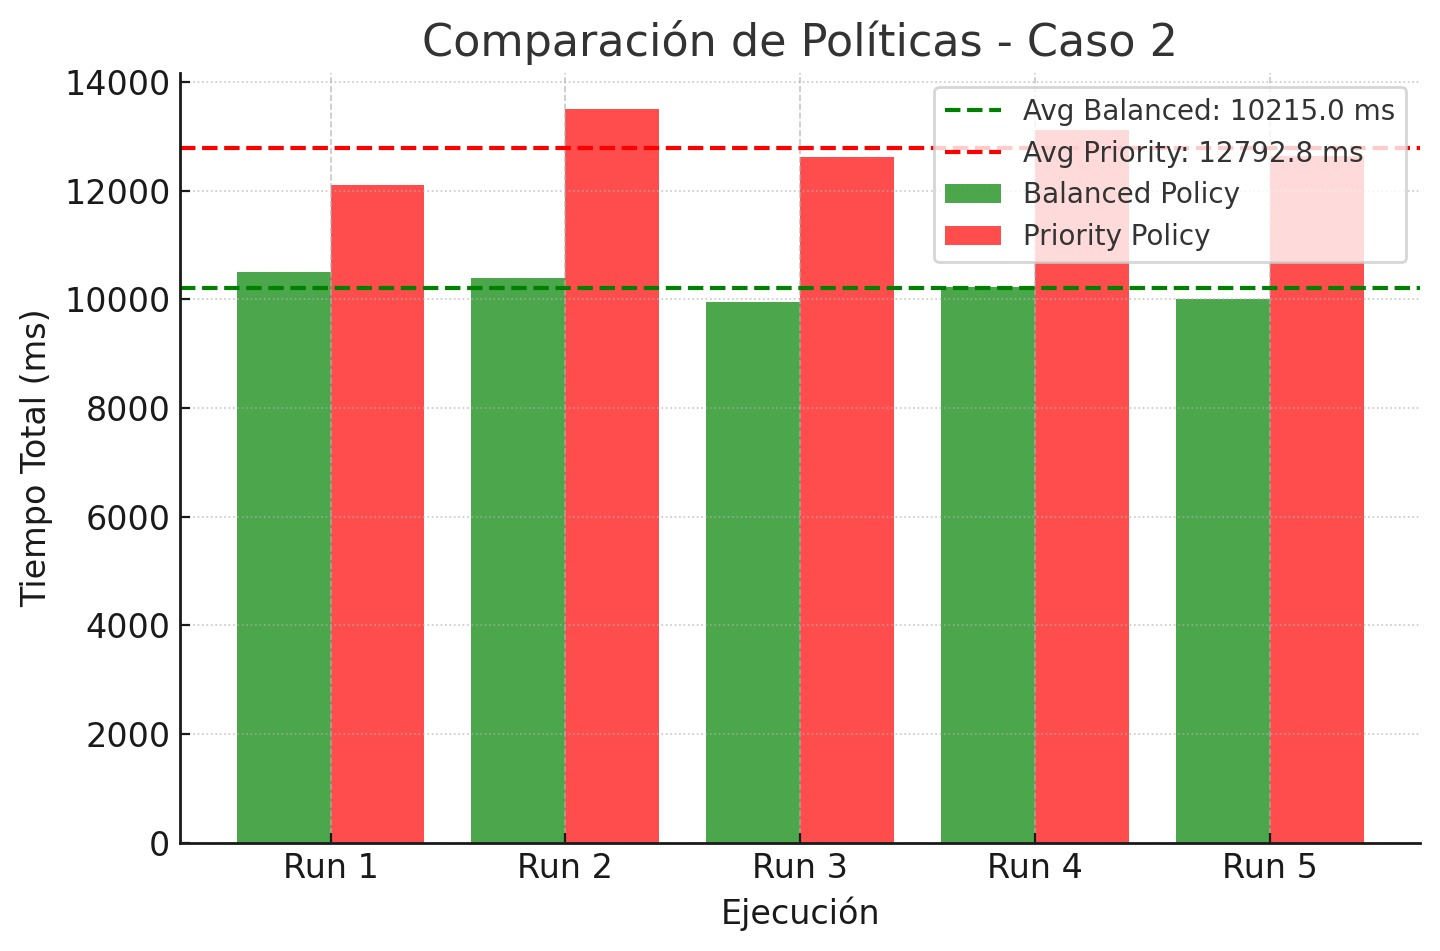
\includegraphics[width=0.7\textwidth]{CASO_2.jpeg}
    \caption{Resultados del Caso 2.}
\end{figure}

En esta configuración, la transición \textbf{Pago} (segmento D) tiene un tiempo de espera mayor. La política \textbf{Priority} favorece \textbf{Pago} con un \textbf{80\%} de probabilidad, lo que incrementa la espera general. Como resultado, el tiempo de ejecución de \textbf{Priority} (\textbf{12792.8 ms}) es mayor que el de \textbf{Balanced} (\textbf{10215 ms}), ya que la estrategia prioritaria selecciona mayormente un camino más lento.

\subsection{Caso 3: Demora en Cancelación y Confirmación de Pago}

\begin{figure}[H]
    \centering
    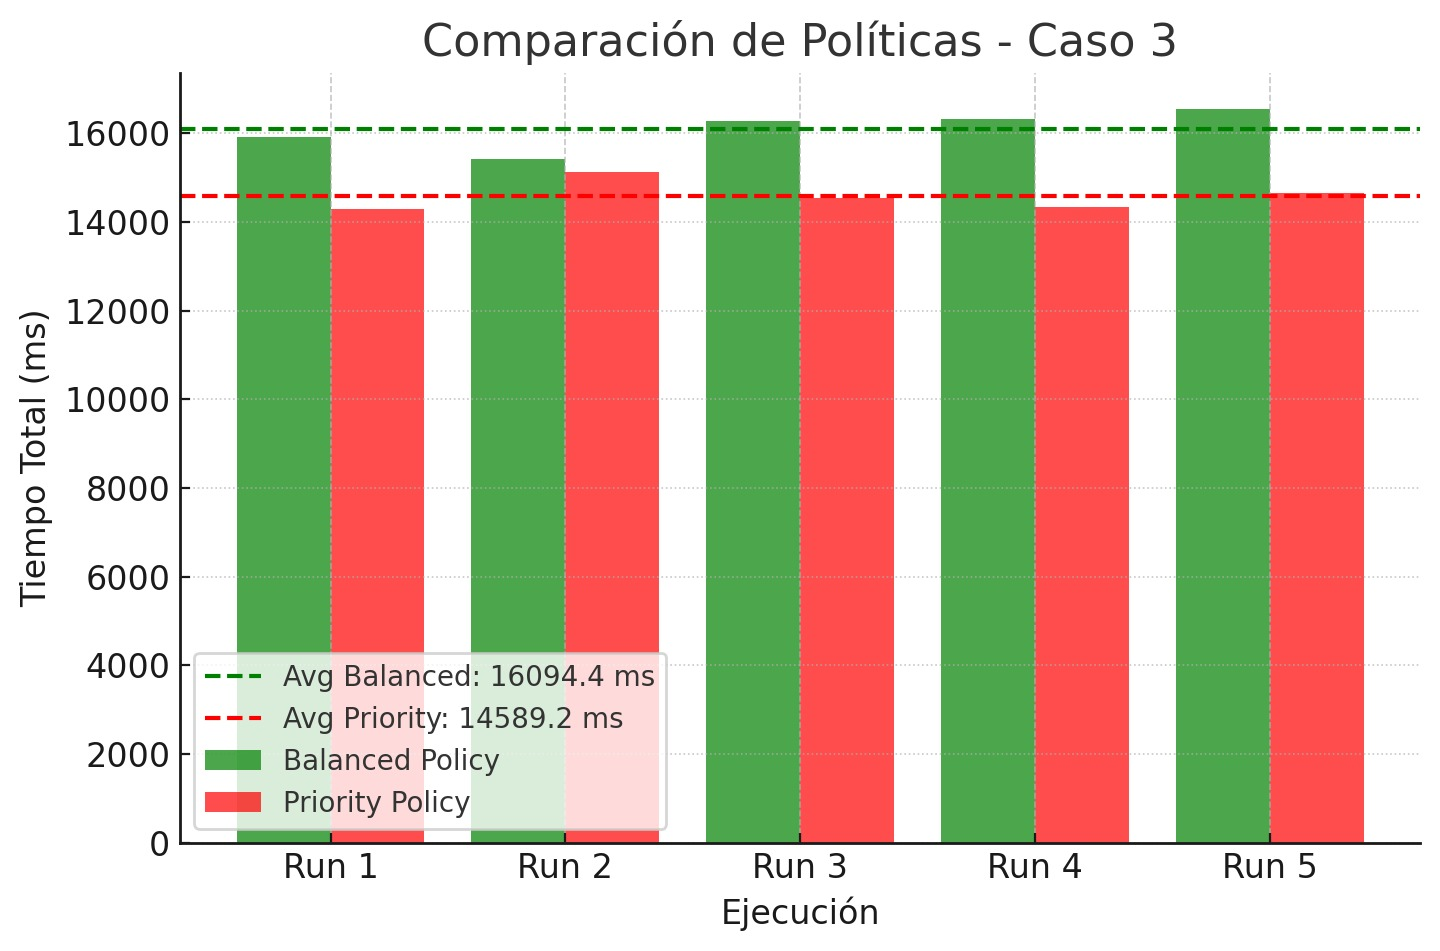
\includegraphics[width=0.7\textwidth]{CASO_3.jpeg}
    \caption{Resultados del Caso 3.}
\end{figure}

En esta configuración, las transiciones \textbf{Cancelación} (segmento E) y \textbf{Confirmación de Pago} (segmento F) tienen \textbf{50 ms} de demora, mientras que las demás solo \textbf{5 ms}. La política \textbf{Priority} evita mayormente \textbf{Cancelación} (20\% de probabilidad) pero no puede evitar \textbf{Confirmación de Pago}, ya que es una transición de cierre del sistema.

Dado que \textbf{Confirmación de Pago} se encuentra en el segmento final, su impacto afecta a ambas políticas por igual. Sin embargo, al reducir el paso por \textbf{Cancelación}, \textbf{Priority} logra un mejor tiempo de ejecución (\textbf{14589.2 ms}) en comparación con \textbf{Balanced} (\textbf{16094.4 ms}).

\subsection{Caso 4: Demora en Reserva Superior y Confirmación de Pago}

\begin{figure}[H]
    \centering
    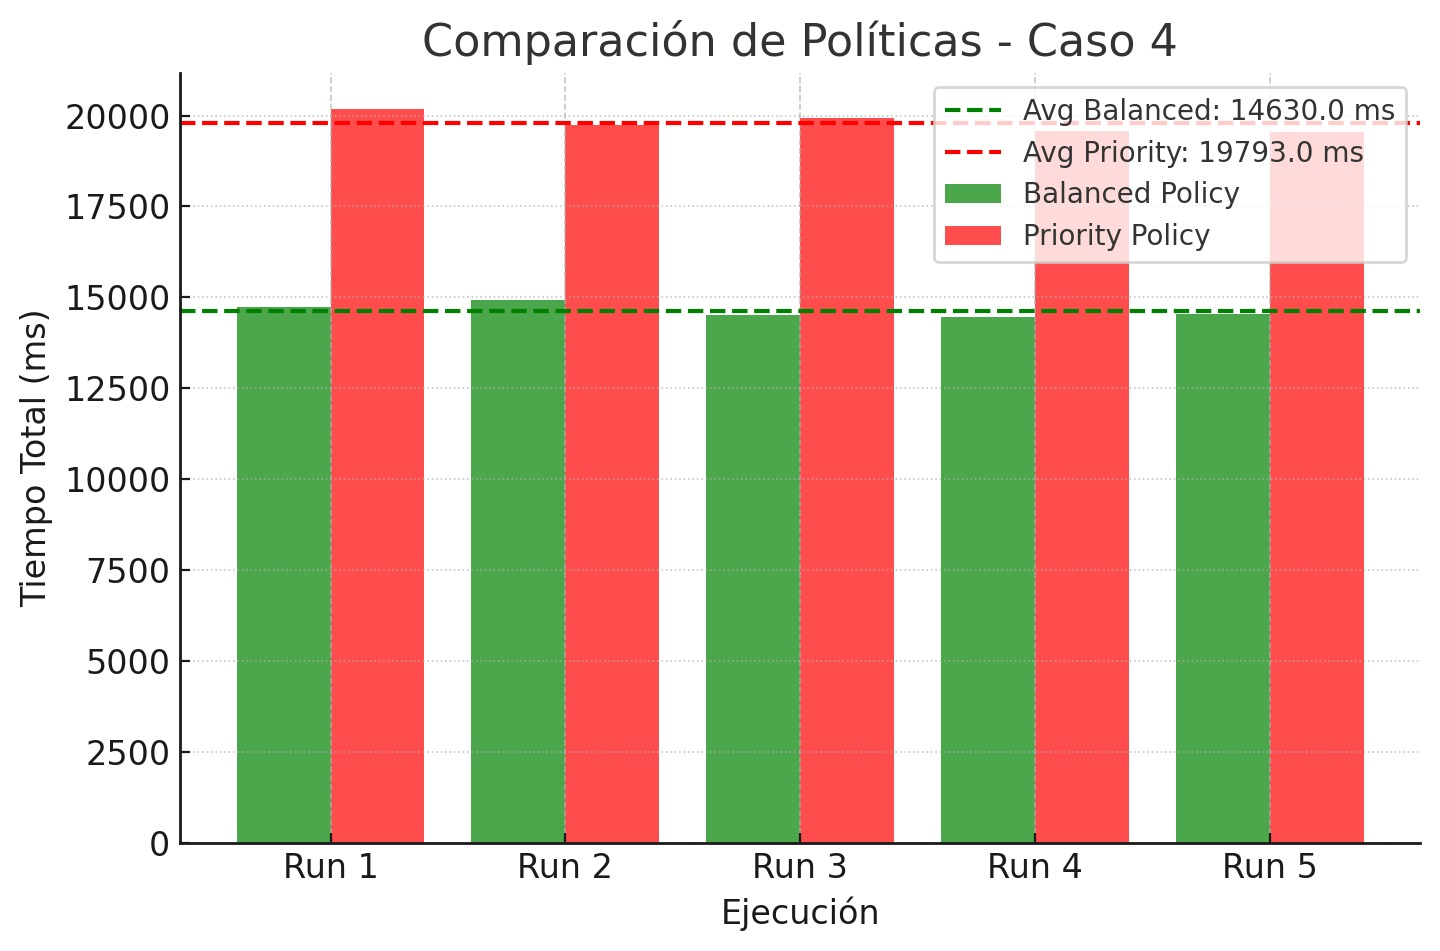
\includegraphics[width=0.7\textwidth]{CASO_4.jpeg}
    \caption{Resultados del Caso 4.}
\end{figure}

Las transiciones \textbf{Reserva Superior} (segmento B) y \textbf{Confirmación de Pago} (segmento F) tienen \textbf{50 ms} de demora. \textbf{Priority} favorece \textbf{B} con \textbf{75\%} de probabilidad, lo que incrementa la espera en este segmento. Como resultado, el tiempo de ejecución con \textbf{Priority} (\textbf{19793 ms}) es significativamente mayor que con \textbf{Balanced} (\textbf{14630 ms}), ya que la estrategia prioritaria no puede evitar los segmentos más lentos.

\subsection{Caso 5: Demora en Ingreso a Sala de Espera}

\begin{figure}[H]
    \centering
    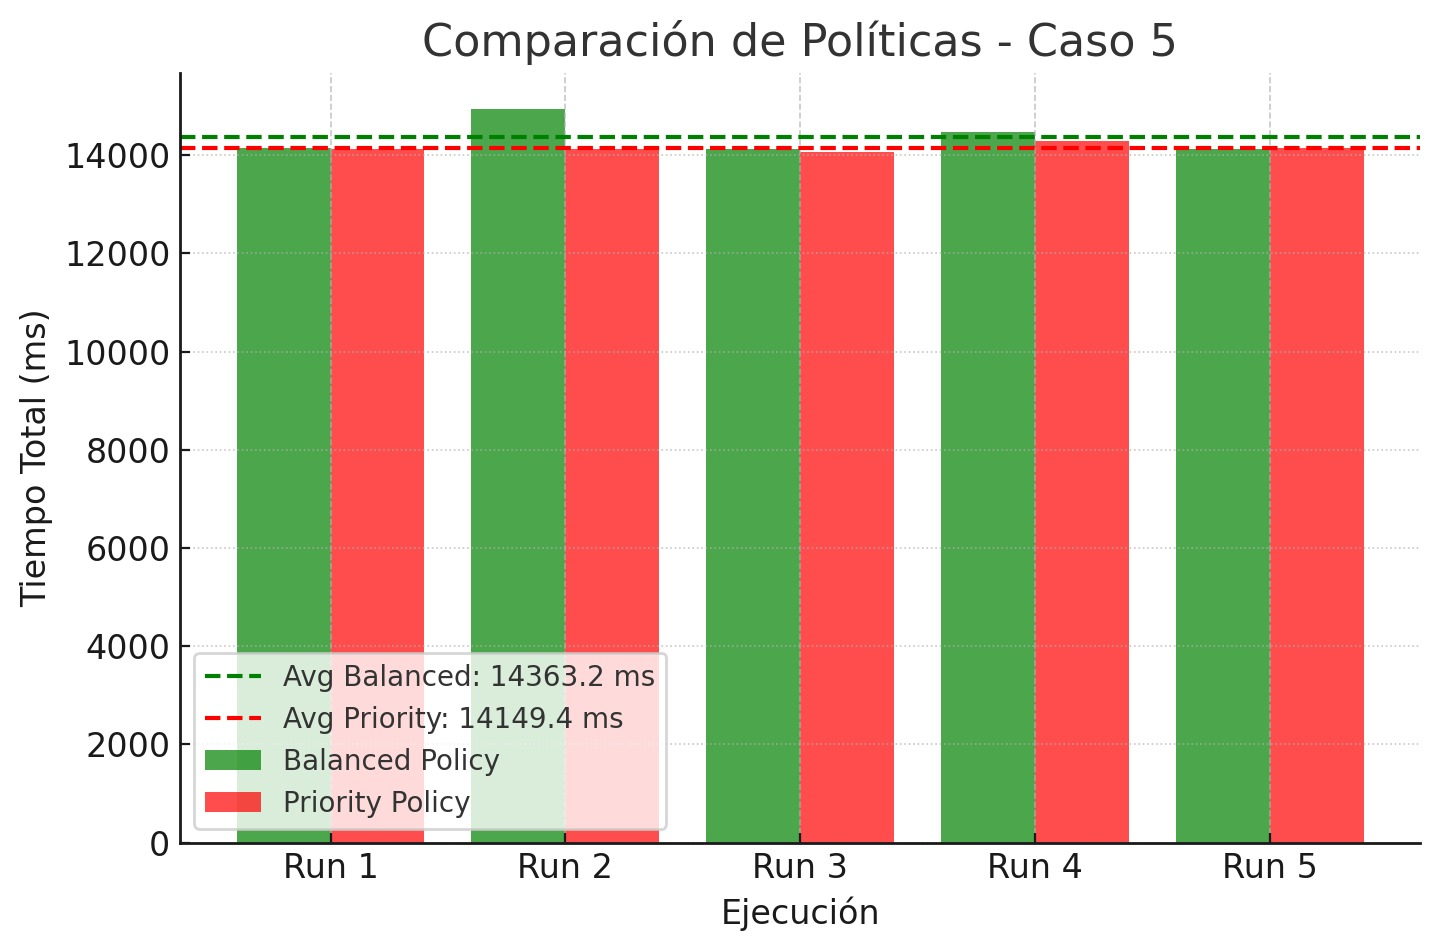
\includegraphics[width=0.7\textwidth]{CASO_5.jpeg}
    \caption{Resultados del Caso 5.}
\end{figure}

Aquí, la transición \textbf{Ingreso a Sala de Espera} (segmento A) tiene \textbf{50 ms} de demora, afectando de manera uniforme a todo el sistema. Esto hace que no haya una gran diferencia entre las políticas, con \textbf{Balanced} obteniendo \textbf{14363.2 ms} y \textbf{Priority} \textbf{14149.4 ms}. Dado que \textbf{Ingreso a Sala de Espera} es el primer paso del sistema, ninguna política puede optimizar su impacto.

\subsection{Caso 6: Demora en Reserva Inferior y Reserva Superior}

\begin{figure}[H]
    \centering
    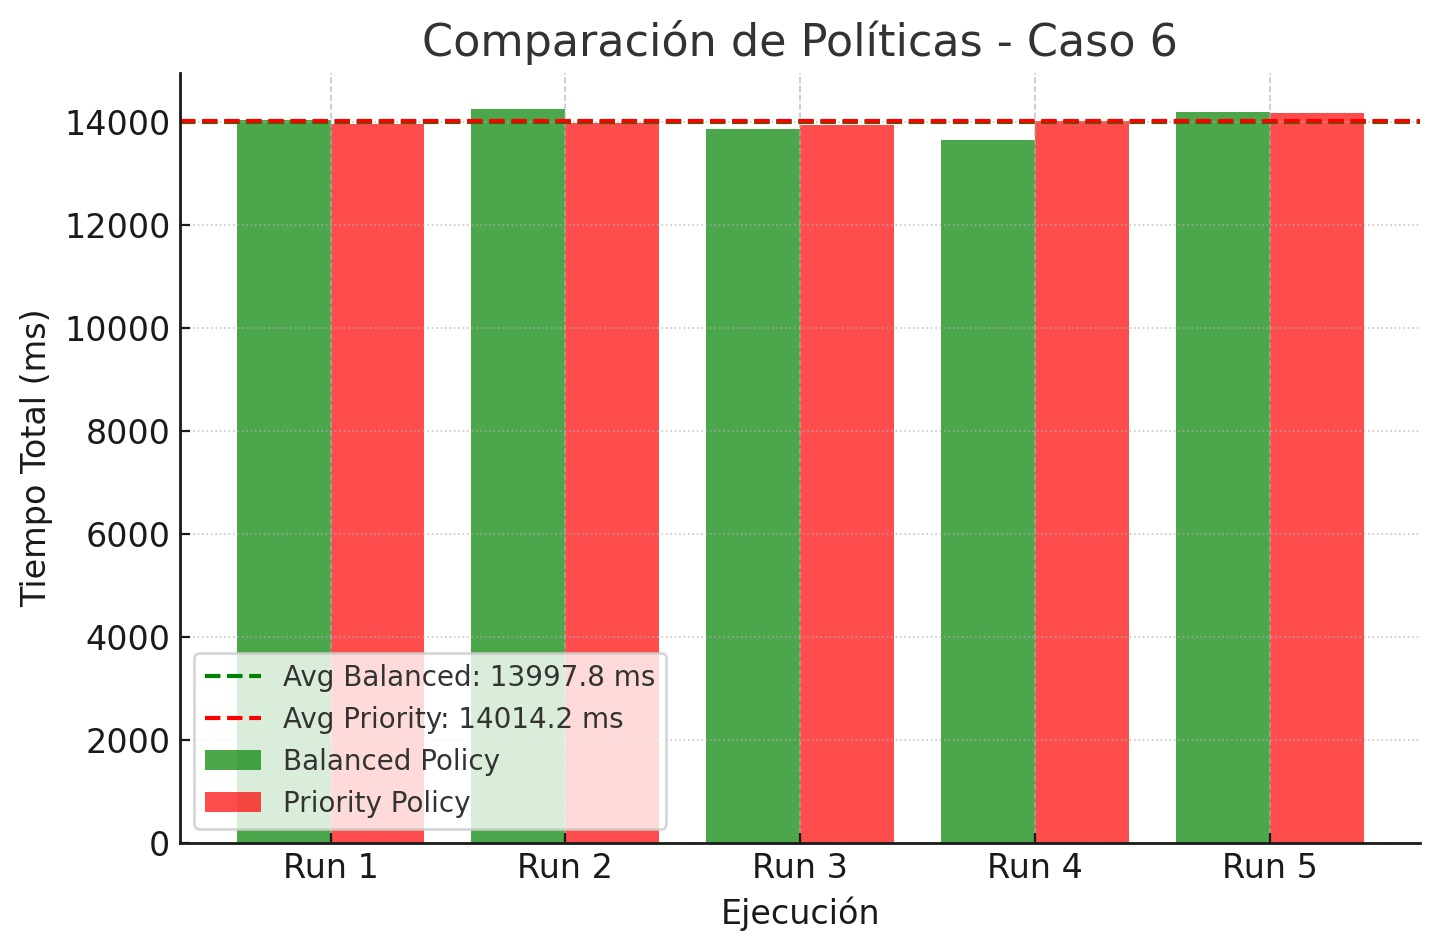
\includegraphics[width=0.7\textwidth]{CASO_6.jpeg}
    \caption{Resultados del Caso 6.}
\end{figure}

Las transiciones \textbf{Reserva Inferior} (segmento B) y \textbf{Reserva Superior} (segmento C) tienen \textbf{50 ms} de demora. Aunque \textbf{Priority} favorece \textbf{B} con \textbf{75\%}, la demora es similar en ambos caminos, lo que hace que el tiempo de ejecución sea casi igual entre ambas políticas (\textbf{Balanced}: \textbf{13997.8 ms}, \textbf{Priority}: \textbf{14014.2 ms}).

\subsection{Caso 7: Demora en Reserva Inferior y Cancelación}

\begin{figure}[H]
    \centering
    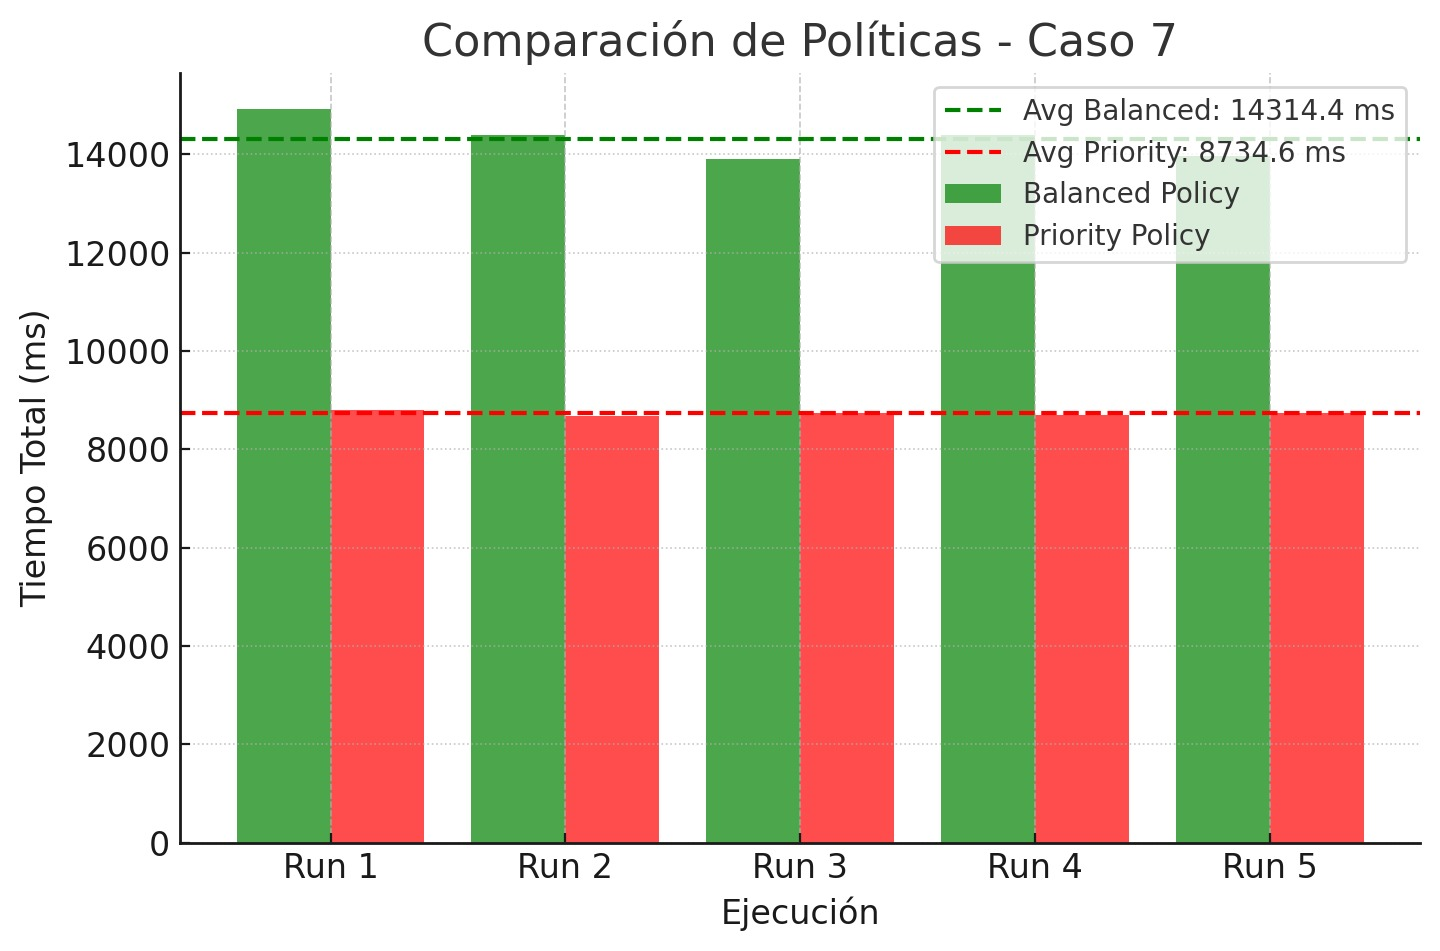
\includegraphics[width=0.7\textwidth]{CASO_7.jpeg}
    \caption{Resultados del Caso 7.}
\end{figure}

En esta configuración, \textbf{Reserva Inferior} (segmento B) y \textbf{Cancelación} (segmento E) tienen \textbf{50 ms} de demora. \textbf{Priority} evita en gran medida \textbf{Cancelación}, favoreciendo \textbf{B} y \textbf{D} en su lugar. Esto hace que \textbf{Priority} sea considerablemente más eficiente (\textbf{8734.6 ms}) que \textbf{Balanced} (\textbf{14314.4 ms}), ya que minimiza la cantidad de ejecuciones que atraviesan \textbf{Cancelación}, reduciendo el impacto del tiempo de espera.

\end{document}
